\chapter{DroneControl}

\section{Introductie} \label{sec:initiele_planning}

In dit hoofdstuk zal besproken worden op welke manier de drone softwarematig wordt aangestuurd.

\subsection{Ontwerpkeuzes}

Het eerste waarover een beslissing moest genomen worden was het al dan niet gebruiken van een reeds bestaande framework, en zoja welke. Bij de keuze van drone werd beschikbaarheid van documentatie reeds in het achterhoofd gehouden waardoor er veel opties beschikbaar waren. Volgende opties werden onderzocht:

\begin{itemize}
\item python-ardrone
\item YADrone
\item AR Drone Simulink Development-Kit
\item AR Drone Toolkit for LabVIEW
\item Nodecopter
\item Parrot SDK
\end{itemize}

Er werd al snel besloten om gebruik te maken van een framework, aangezien er hierdoor meer tijd kan gestoken worden in de eigenlijke projectdoelstellingen. De meeste frameworks vielen ook al meteen af aangezien ze niet voldoende gedocumenteerd waren of gebruik maakten van software en/of programmeertaal waarmee we niet voldoende vertrouwd mee waren. De laatste keuze moest gemaakt worden tussen de python framework en Nodecopter. Doorslaggevend voor de keuze voor Nodecopter was de zeer grote beschikbaarheid van documentatie en extra modules. Aangezien er via Python werd gecommuniceerd zorgde dit er wel voor dat de droneControl moest worden opgesplitst in twee delen. Eenerzijds het Nodejs deel dat de commando's doorstuurt naar de drone, en anderzijds het python script dat de positie zal ophalen van de mqqt server. Tot slot moest er nog besloten worden in welk van de twee delen de positie verwerkt zou worden naar een commando dat doorgegeven kan worden aan de drone. Hiervoor is python gekozen aangezien we hier meer ervaring mee hebben.




\section{Communiceren met de drone via Nodecopter}


Aangezien alle berekeningen reeds worden gedaan in het Python script is de node kant niet veel meer dan een tussenstuk dat alle data ontvangt op een lokale socket en direct doorstuurt naar de drone door middel van Nodecopter commands. Het enige andere nog vernoemenswaardige feature is dat het script ook de hoogte zal ontvangen van de drone en dit terugsturen over dezelfde socket. Dit gebeurd parallel aan de besturingslus zodanig deze niet moet staan wachten op niet triviale hoogte data.\\

We gebruiken de 'node-ar-library' van Nodecopter. Dit is de standaard library voor het besturen van de drone. Deze laat toe om de drone high level aan de sturen. Er kan simpelweg een drone object worden aangemaakt waarop functies als 'forward' of 'left' kunnen opgeroepen worden met als argumenten een fractionele snelheid tussen 0 (stil) en 1 (maximum snelheid). Voor andere richtingen in het 3-dimensioneel vlak bestaan gelijkaardige commands. Rotatie gebeurt ook gelijkaardig, met een hoeksnelheid tussen -1 en 1.\\

Het gebruik van de 'ardrone-autonomy' library werd ook onderzocht. Dit is een uitbreiding op de standaard library die toelaat om de drone nog meer high level aan te sturen aan de hand van afstand en draaihoek in plaats van snelheid. Al snel werd echter duidelijk dat voor binnenvluchten met kleinere foutmarges deze library niet accuraat genoeg is. Dit komt doordat de drone geen ingebouwde gps heeft, en zijn relatieve positie dus enkel maar kan baseren op het geleverde vermogen aan de motoren, wat verre van accuraat is.



\begin{figure}[h]
\caption{Een flowchart van het Nodescript}
\centering
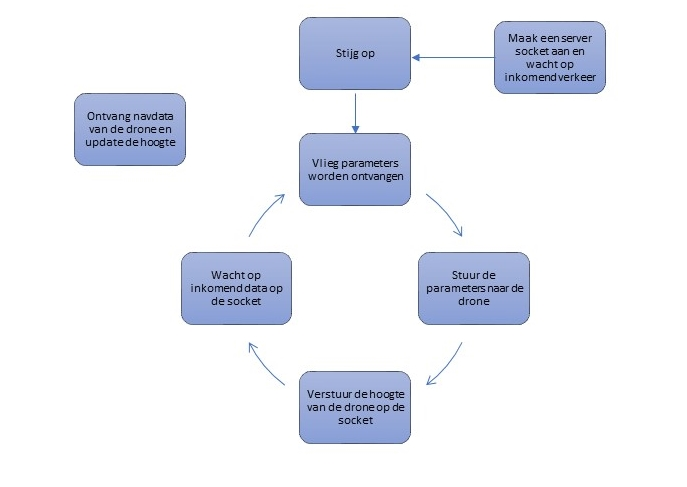
\includegraphics[width=\textwidth]{images/node_server_flowchart}
\end{figure}

\section{Verwerken van de data in Python}


Het Python script doet het meeste van het werk. De locatie vanop de mqtt server wordt gebruikt om te berekenen tegen welke snelheid en in welke richting de drone moet vliegen. Deze informatie wordt dan doorgestuurd over een lokale socket naar het Node.js script op poort 8124.

\begin{figure}[h]
\caption{Een flowchart van het Nodescript}
\centering
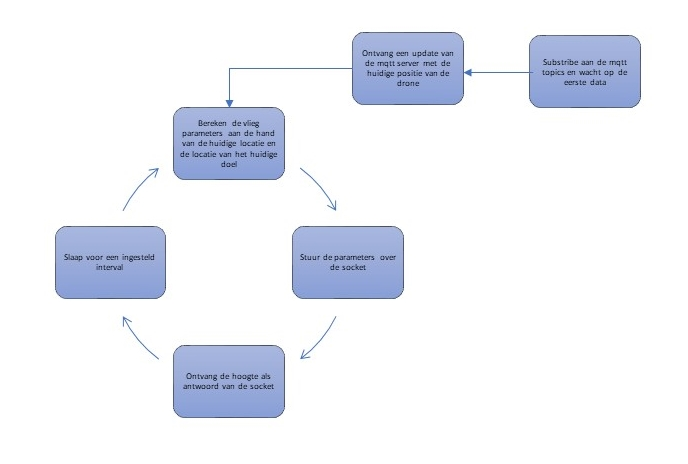
\includegraphics[width=\textwidth]{images/python_client_flowchart}
\end{figure}

\subsection{Vliegalgoritme 1}

Een eerste poging bestond eruit de info omtrent de locatie te gebruiken en om te zetten in twee snelheden, namelijk een voorwaartste snelheid en een hoeksnelheid. Het idee was simpel: de drone draait zich telkens in de juist richting en gaat dat vooruit. Hoewel dit idee theoretisch goed klinkt was dit praktisch moeilijker uit te voeren. Een eerste probleem was dat het vooruit vliegen en draaien parallel gebeurde, wat er dus voor zorgde dat de drone eerder in een boog vloog in plaats van rechtdoor. Dit kon eventueel verholpen worden door de twee acties sequentieel uit te voeren, maar op die manier zouden we nog een nieuwe timing afhankeijkheid creeren (Wat als de drone nieuwe vliegdata ontvangt maar hij is nog bezit met draaien?), en dat leek ons suboptimaal. 

\subsection{Vliegalgoritme 2}

In een tweede poging werd enkel gebruik gemaakt van de lineare richtingen van de drone, en niet geroteerd. Het komt er dus op neer dat de drone enkel naar voor, achter, link of rechts gaat, en zijn 'oog' steeds naar dezelfde kant wijst. Dit bleek een accurater algoritme dus hebben we dit verder uitgewerkt. Een grote beperking in de set up is dat de hoek berekend d.m.v. de pozyx tags relatief is, en bij elke opstart anders is. Dit heeft als gevolg dat de drone telkens gealligneerd met het assenstelsel moet opstijgen. Ook hier neemt de snelheid linear af, tot de drone binnen een gegeven afstand van het punt is. Dan zet hij de 'done' parameter op true, en kan er over gegaan worden naar het volgende punt in de lijst.

\section{Gebruik}

\subsection{Lijst van afhankelijkheden}

Python:\\
paho-mqtt\footnote{\url{https://pypi.org/project/paho-mqtt}}\\
pypozyx\footnote{\url{https://github.com/pozyxLabs/Pozyx-Python}}\\
\\
Node.js:\\
ar-drone\footnote{\url{https://github.com/felixge/node-ar-drone}}\\

\subsection{Configuratie}

In de config.json file kunnen verschillende parameters worden ingesteld voor het gebruiken en testen van de code. \\

\begin{tabular}{ l | l }
IP & Het IP adress van de mqqt server\\
PORT & De poort gebruikt door de mqqt server\\
topic\_x & De naam van de topic op de mqqt server die x published\\
TIME\_INTERVAL & De tijd dat er geslapen wordt tussen het sturen van commands (s)\\
MAX\_SPEED & De maximale snelheid die naar de drone kan gestuurd worden t.o.v. zijn absoluut maximum (0..1)\\
POSITION\_THRESHOLD & De straal van de cirkel waarbinnen de drone een punt als 'bereikt' ziet (mm)\\
MAX\_ROTATION & De maximale rotatiesnelheid die naar de drone kan gestuurd worden t.o.v. zijn absoluut maximum (0..1)\\
ROTATION\_THRESHOLD & Marge op de hoek waarbinnen niet gecorrigeerd wordt (graden)\\
\end{tabular}




\subsection{Starten}


Start de pozyx tag.\\
Maak verbinding met de drone over wifi.\\
start \textit{server.js}, dit zal verbinding maken met de drone en wachten op socketverkeer.\\
start \textit{client.py}, dit zal verbinding maken met de mqqt server en beginnen vliegdata over de socket te sturen.\\
